
\documentclass[12pt]{article}
\usepackage{graphicx}

%%%%%%%%%%%%%%%%%%%%%%%%%%%%%%%%%%%%%%%%%%%%%%%%%%%%%%%%%%%%%%%%%%%%
% basic data for the eprint:
%%%%%%%%%%%%%%%%%%%%%%%%%%%%%%%%%%%%%%%%%%%%%%%%%%%%%%%%%%%%%%%%%%%%

\textwidth=6.0in  \textheight=8.25in

%%  Adjust these for your printer:
\leftmargin=-0.3in   \topmargin=-0.20in

%% preprint number data:
\newcommand\pubnumber{}
\newcommand\pubdate{\today}

%%  address and funding acknowledgement data:
\def\institute{Centre for Cosmology, Particle Physics and Phenomenology\\
Universit\'e catholique de Louvain, B-1348 Louvain-la-Neuve, BELGIUM}
\def\support{\footnote{Work supported by Fonds de la Recherche Scientifique (FNRS), Belgium.}}

%%%%%%%%%%%%%%%%%%%%%%%%%%%%%%%%%%%%%%%%%%%%%%%%%%%%%%%%%%%%%%%%%%%%%%%%%%%%
%   document style macros
%%%%%%%%%%%%%%%%%%%%%%%%%%%%%%%%%%%%%%%%%%%%%%%%%%%%%%%%%%%%%%%%%%%%%%%%%%%%
\def\Title#1{\begin{center} {\Large #1 } \end{center}}
\def\Author#1{\begin{center}{ \sc #1} \end{center}}
\def\Address#1{\begin{center}{ \it #1} \end{center}}
\def\andauth{\begin{center}{and} \end{center}}
\def\submit#1{\begin{center}Submitted to {\sl #1} \end{center}}
\newcommand\pubblock{\rightline{\begin{tabular}{l} \pubnumber\\
         \pubdate  \end{tabular}}}
\newenvironment{Abstract}{\begin{quotation}  }{\end{quotation}}
\newenvironment{Presented}{\begin{quotation} \begin{center} 
             PRESENTED AT\end{center}\bigskip 
      \begin{center}\begin{large}}{\end{large}\end{center} \end{quotation}}
\def\Acknowledgements{\bigskip  \bigskip \begin{center} \begin{large}
             \bf ACKNOWLEDGEMENTS \end{large}\end{center}}
%%%%%%%%%%%%%%%%%%%%%%%%%%%%%%%%%%%%%%%%%%%%%%%%%%%%%%%%%%%%%%%%%%%%%%%%%%%%
%  personal abbreviations and macros
%    the following package contains macros used in this document:
\input econfmacros.tex
%%%%%%%%%%%%%%%%%%%%%%%%%%%%%%%%%%%%%%%%%%%%%%%%%%%%%%%%%%%%%%%%%%%%%%%%%%%

\begin{document}
\begin{titlepage}
\pubblock

\vfill
\Title{Measurements of single top quark cross sections at 13~TeV with the CMS experiement}
\vfill
\Author{Matthias Komm\support}
\Address{\institute}
\vfill
\begin{Abstract}
An overview of recent measurements of inclusive and differential single top quark cross sections at 13~TeV with the CMS experiment is given in the following. t/tdiff/tw,tzq
\end{Abstract}
\vfill
\begin{Presented}
$10^{th}$ International Workshop on Top Quark Physics\\
Braga, Portugal,  September 17--22, 2017
\end{Presented}
\vfill
\end{titlepage}
\def\thefootnote{\fnsymbol{footnote}}
\setcounter{footnote}{0}
%

\section{Introduction}


\section{Cross sections in $t$~channel}

\section{Single top quark production in association with a W~boson}

\section{Single top quark production in association with a Z~boson}

\section{Conclusion}

\begin{figure}[!htb]
\begin{center}
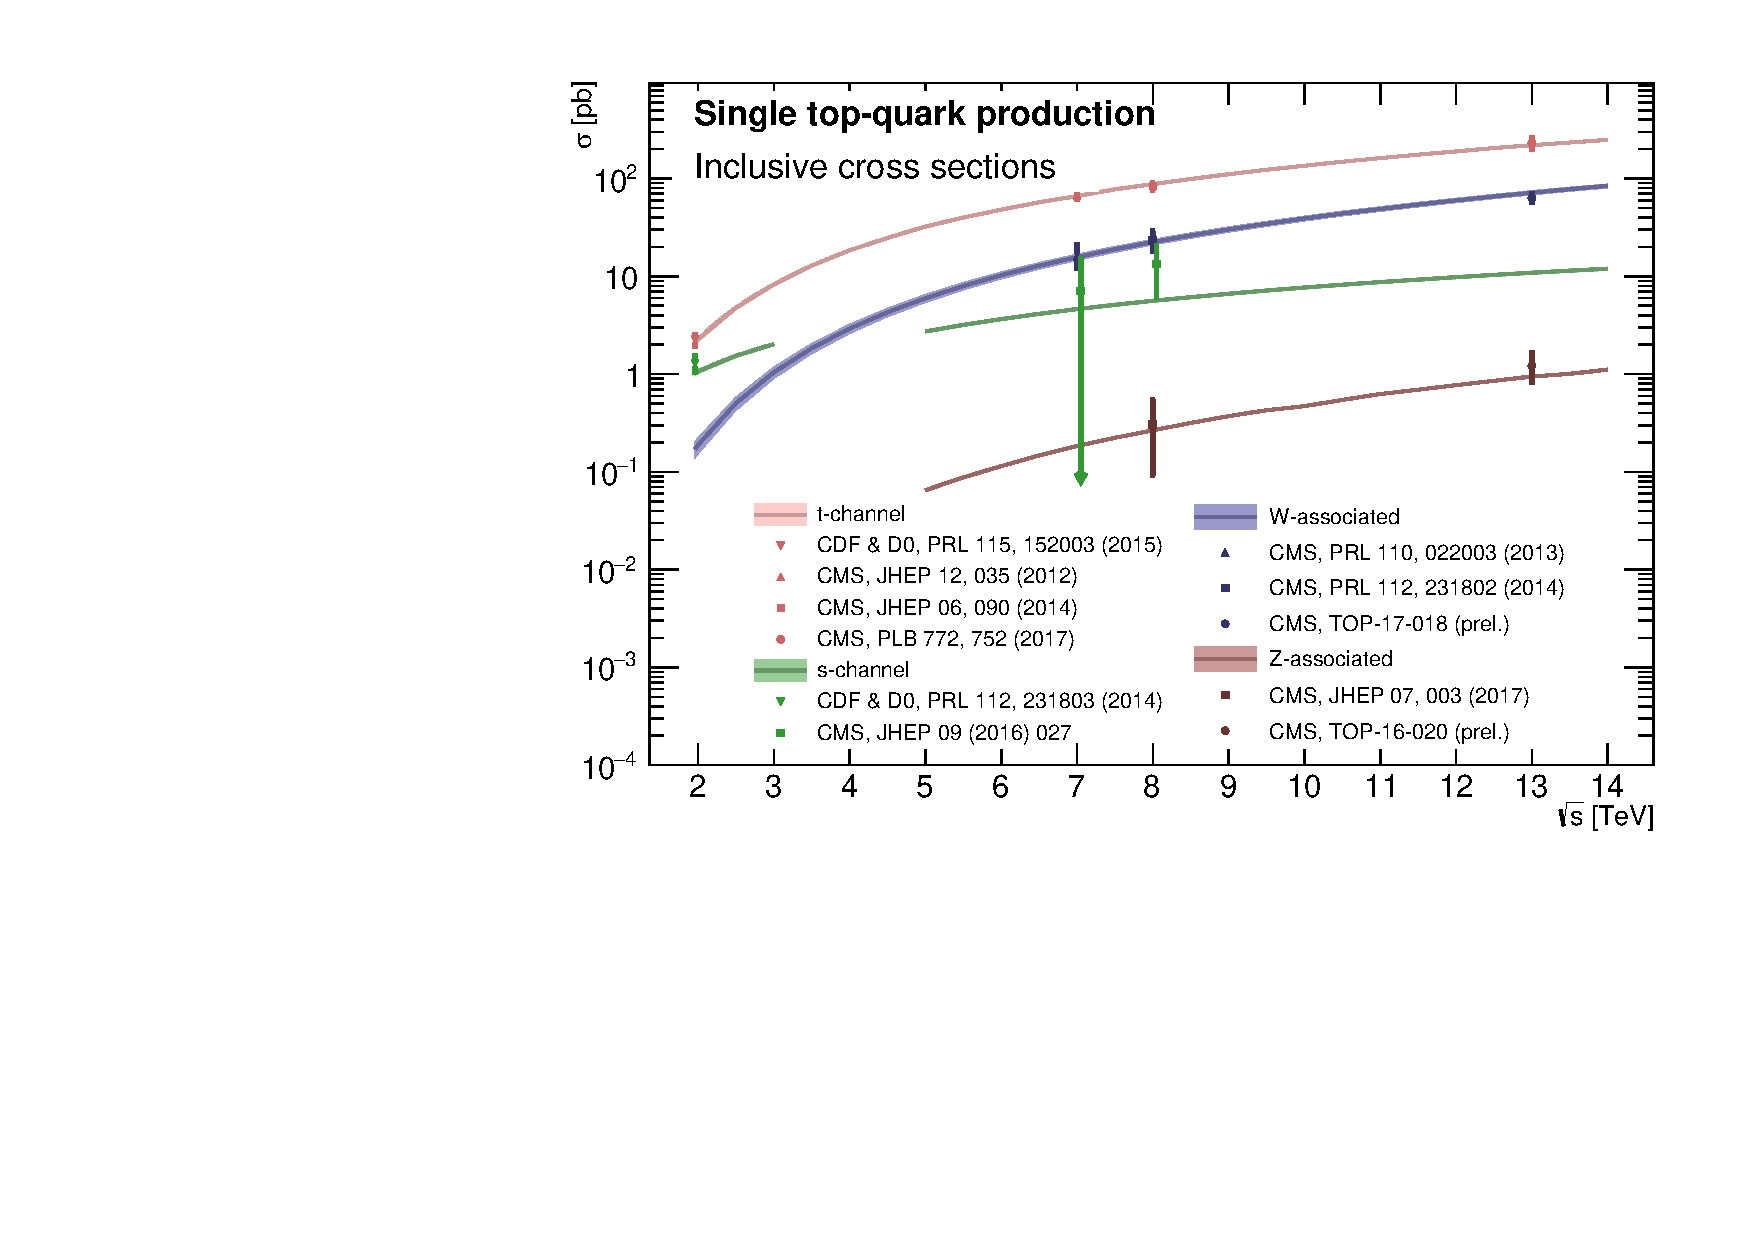
\includegraphics[width=0.7\textwidth]{singletopSep2017_noATLAS.pdf}
\caption{Overview of inclusive single top quark cross section measurements with the CMS experiment. The figure is adapted from Ref.~\cite{Giammanco}.}
\end{center}
\end{figure}

\begin{thebibliography}{99}

\bibitem{Giammanco}{A. Giammanco and R. Schwienhorst, arXiv:1710.10699 [hep-ex].}

\bibitem{Mesmer}{F. A. Mesmer, Proc. Wien. Acad. Sci. {\bf 13}, 1564, 1593 (1762).}

\end{thebibliography}

 
\end{document}

